% ----------------------------------------------------------------------------
% Copyright (c) 2016 by Burkhardt Renz. All rights reserved.
% Die Vorlage für eine Abschlussarbeit in der Informatik am Fachbereich
% MNI der THM ist lizenziert unter einer Creative Commons
% Namensnennung-Nicht kommerziell 4.0 International Lizenz.
%
% Id:$
% ----------------------------------------------------------------------------

\chapter{Problembeschreibung}
\label{chapter:Problembeschreibung}
\section{Eventgenerierung}
\label{section:Eventgenerierung}


\begin{figure}[!ht]
	\centering
	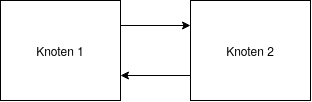
\includegraphics[scale=0.5]{img/synchronisation/distributed_system_application_minimal.png}
	\caption[Minimale Struktur eines verteilten Systems]{Minimale Struktur eines verteilten Systems, bestehend aus zwei Komponenten}
	\label{fig:distributed_system_application_minimal}
\end{figure}

Wir definieren ein minimales verteiltes System, bestehend aus zwei Komponenten. \cref{fig:distributed_system_application_minimal} bildet ein solches System ab. Die Knoten beinhalten zwei für distributed tracing interessante Aspekte. Dies ist zum einen die verteilte Anwendung mit ihrem instrumentalisiertem Code und zum Anderen das Netzwerk, über welches Nachrichten ausgetauscht werden.

\begin{figure}[!ht]
	\centering
	\begin{subfigure}[t]{.49\linewidth}
		\centering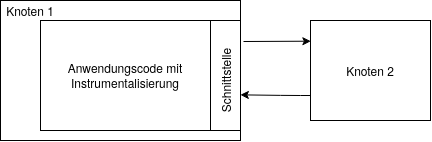
\includegraphics[width=0.9\linewidth]{img/synchronisation/distributed_system_application_inside.png}
		\caption[Abbildung]{zeigt Knoten mit instrumentalisiertem Anwendungscode}
		\label{fig:distributed_system_application_inside}
	\end{subfigure}
	\begin{subfigure}[t]{.49\linewidth}
		\centering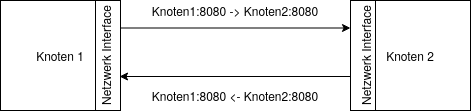
\includegraphics[width=\linewidth]{img/synchronisation/distributed_system_network.png}
		\caption[Abbildung]{Netzwerkkommunikation über TCP/IP}
		\label{fig:distributed_system_network}
	\end{subfigure}
	\caption[Anwendungsinstrumentalisierung und Netzwerkkommunikation über TCP/IP in verteilten Systemen]{}
\end{figure} 

\subsection{Eventkorrelation}
\label{subsection:Eventkorrelation}
\subsection{Synchronistion von Eventgeneratoren}
\label{subsection:Synchronistion von Eventgeneratoren}
\section{Eventübermittlung}
\label{section:Eventübermittlung}

% ----------------------------------------------------------------------------
